\documentclass[10pt,a4paper]{article}
\usepackage[left=2cm,right=2cm,top=2cm,bottom=2cm]{geometry}
\usepackage[dvipsnames]{xcolor}
\usepackage[fleqn]{mathtools}
\usepackage{booktabs}
\usepackage{amsmath}
\usepackage{latexsym}
\usepackage{graphicx}
\usepackage{nccmath}
\usepackage{multicol}
\usepackage{listings}
\usepackage{tasks}
\usepackage{color}
\usepackage{float}
\usepackage{lipsum}

\definecolor{colorIPN}{rgb}{0.5, 0.0,0.13}
\definecolor{colorESCOM}{rgb}{0.0, 0.5,1.0}
\graphicspath{ {imagenes/} }

\begin{document}
%#########################################################
\begin{titlepage}
	\centering
	{ \huge \bfseries \color{colorIPN}{Instituto Politécnico Nacional} \par}
	{ \Large \bfseries  \color{colorESCOM}{Escuela Superior de Cómputo} \par }
	\vspace{1cm}
	{\huge\Large \color{colorIPN}{Web App Development}.\par}
	\vspace{1.5cm}
	{\huge\Large  \color{colorESCOM}{Practica 2: JSP.}\par}
		\vspace{2cm}
	{\Large\itshape \color{colorIPN}{Profesor: M. en C. José Asunción Enríquez Zárate }\par} \hfill \break
	\vspace{2cm}
	{\Large\itshape \color{colorIPN}{Alumno: Chavarría Vázquez Luis Enrique}\par} \hfill \break
	{\Large\itshape \color{colorIPN}{luisechvz@gmail.com}\par} \hfill \break
	{\Large\itshape \color{colorIPN}{3CM4} \par}
	\vfill
	{\large \color{colorIPN}{\today}\par} 
	\vfill
\end{titlepage}

\renewcommand\lstlistingname{Quelltext} 


\lstset{ 
	language=Java,
	basicstyle=\small\sffamily,
	numbers=left,
	numberstyle=\tiny,
	frame=tb,
	tabsize=4,
	columns=fixed,
	showstringspaces=false,
	showtabs=false,
	keepspaces,
	commentstyle=\color{Violet},
	keywordstyle=\color{colorIPN} \bfseries,
	stringstyle=\color{colorESCOM}
}

\settasks{
	counter-format=(tsk[r]),
	label-width=4ex
}
\tableofcontents 
\pagebreak
\listoffigures
\pagenumbering {arabic}

\pagebreak

%################################################
\section{\color{colorIPN}{Introducción}}

Durante el desarrollo de esta práctica, podemos apreciar como hemos hecho una implementación de un sistema gestor de categorías por medio del uso de la tecnología del lenguaje de programación JAVA y la implementación de lo ya populares JSP, con lo cual a lo largo de esta práctica podremos apreciar de forma detallada como hemos hecho la implementación de múltiples opciones como la el cual puede ser tener una página de bienvenida, agregar categorías, actualizar las categorías, eliminar las categorías, poder visualizar las categorías con todas información y ademas de ello mostrar un mensaje de error en caso de que sea necesario y se requiera en algun momento de la ejecución del programa.

\vspace{5mm}

A decir verdad este es una de las mejores prácticas queremos hecho ya que hemos podido apreciar de forma muy precisa como se ha realizado el implementación del sistema y ademas de ello hemos tenido la oportunidad de poder personalizar nuestra interfaz para poder ofrecer una mejor experiencia de usuario, con lo cual se complementan ambas partes en la cual trabajamos con base de datos pero también estamos trabajando con la parte de la interfaz que el usuario observa cuando utiliza en interactúa con nuestro sistema, con lo cual podemos darnos cuenta de que toda la implementación realizada y que a continuación se mostrará cumple de manera contundente con los propósitos del curso además de que en mi opinión se ha podido ver una aplicación realmente practica en el desarrollo de esta práctica y hemos aprendido que mis caminos llevan a Roma, a lo que me refiero con esto es que hemos hecho la implementación de nuestra base datos la conexión de la base datos con nuestro código de una forma un poco diferente configurando directamente nuestro servidor, pero no por esto debemos menospreciar la práctica ya que al hacerlo de forma diferente podemos aprender diversas formas de poder implementar nuestros proyectos y podrá trabajar con ellos de manera más dinámica y desde luego bajo ciertas circunstancias en las que podríamos vernos involucrados en algun desarrollo de algun software que evidentemente requiera que nosotros trabajemos con las circunstancias y con las características que el cliente nos está especificando o que el mismo equipo de desarrollo está requiriendo como por lo cual puedo afirmar que en esta práctica realmente sí se exploran otras opciones para poder desarrollar algo muy similar a lo que habíamos aplicado la practica número uno, pero ahora viéndolo desde una perspectiva diferente para poder entender las ventajas y desventajas que una u otra implementación pueden tener frente a otras que probablemente ya conocíamos, con lo cual uno no se queda estancado siempre lo mismo y puede seguir avanzando.

\vspace{5mm}

Desde luego uno de los aspectos en los que nos enfocaremos en en desarrollo y reporte de esta práctica, ese trabajo precisamente con la parte de la interfaz y también mostraron poco sobre como es que funciona nuestra base datos y explicar de forma General y en términos muy concretos como es que código está estructurado para poder hacer que todo el sistema funcione en armonía y de forma totalmente satisfactoria de acuerdo a las necesidades que establecimos en un principio, con lo cual se cumple mostrar todas las funciones y también poder generar una experiencia al usuario bastante buena al momento interactuar con ese interfaz ya que hemos utilizado herramientas o frameworks que actualmente están disponibles en el mercado y que se acoplan de manera magistral a nuestro desarrollo ya sea de manera local o de manera online por medio del uso de las CDN’s. Entonces sin más por el momento o damos inicio a la práctica número dos.


\pagebreak

%################################################
\section{\color{colorIPN}{Conceptos (generalidades)}}

\subsection{JSP.}
Directiva JSP para ajustar toda la página JSP relacionados atributos, tales como la página de codificación y lenguajes de script. Las instrucciones pueden tener una serie de propiedades, que en forma de pares de clave y valor, separados por comas.

\subsection{Declaraciones.}
Las declaraciones se utilizan para declarar variables o métodos dentro de un JSP, de igual forma que se haría dentro del código Java de un servlet tradicional.

\subsection{SERVLETS.}
Un servlet es una clase en el lenguaje de programación Java, utilizada para ampliar las capacidades de un servidor. El uso más común de los servlets es generar páginas web de forma dinámica a partir de los parámetros de la petición que envíe el navegador web.

\subsection{Scriptlets.}
Permiten ejecutar código arbitrario, cuyo resultado no es necesario enviar a la salida. Si desde un scriptlet se desea escribir algo en ésta, bastará con utilizar el objeto predefinido out. Un uso común de los scriptlets es hacer que ciertas partes de código HTML aparezcan o no en función de una condición.

\subsection{Expresiones.}
Una expresión es una sentencia Java que es evaluada y cuyo resultado es convertido a texto siguiendo las reglas habituales de conversión. La cadena de texto resultante es añadida directamente a la respuesta de la petición a través del Writer, de igual forma que se haría por código dentro de un servlet tradicional.

\subsection{Aplicación web.}
En la Ingeniería de software se denomina aplicación web a aquellas aplicaciones que los usuarios pueden utilizar accediendo a un Servidor web a través de Internet o de una intranet mediante un navegador.

\subsection{JDBC.}
JDBC proporciona Controladores JDBC que convierte la solicitud de la aplicación Java en el lado del cliente al lenguaje que entiende la base de datos. Como JDBC es específico del idioma y la plataforma, la aplicación Java puede usar JDBC a ODBC puente para comunicarse con bases de datos adaptables ODBC.


\pagebreak

%################################################
\section{\color{colorIPN}{Desarrollo}}
En esta primera imagen podemos apreciar toda la estructura y el directorio Home nuestro proyecto, el cual está corriendo a través del entorno de desarrollo o IDE Netbeans, el cual nos ofrece una robustas tremenda para poder trabajar con proyectos de distintas gamas y paridades, por lo cual en este proyecto nos abocaremos precisamente a una aplicación web pero con el enfoque que ya hemos mencionado previamente en la introducción a nuestro proyecto con lo cual estará sujeta algunos cambios respecto a la práctica uno que ya habíamos visto o de manera previa en clases anteriores en las cuales se trató o tanto el aspecto teórico como el aspecto práctico todo de manera dual y paralela.

\begin{figure}[h]
\centering
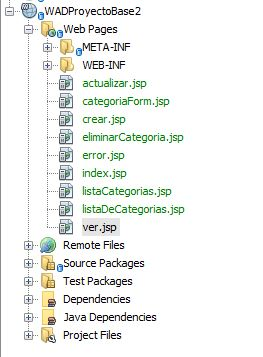
\includegraphics[width=5cm]{1}
\caption{Imagen 1.}
\label{fig:figure1}
\end{figure}

Primero que nada antes de entrar de lleno en el código, vale la pena destacar que necesitamos primero visualizar como quedó la aplicación y como es que la interfaz se ve directamente para poder entender de posteriormente que estamos describiendo y como es que cada una de estas partes funcionar en su conjunto, por lo cual desde mi perspectiva parece más conveniente poder analizar primero la parte visual y la parte que el usuario tiene frente a su pantalla y posteriormente ahondar con mucho más detalle en todo lo que está detrás tanto o a nivel frontend como nivel backend, por lo cual como lo he mencionado en esta primera imagen que podemos apreciar se de la página de bienvenida, la cual implementa precisamente el paradigma de diseño de Google material design el cual hasta hoy por hoy representa un estándar para el industria y sobre todo para el entorno de aplicaciones móviles pero también para muchas de las páginas web que actualmente circulan en internet, por lo cual es un paradigma de diseño bastante dinámico además de que nos ofrece muchísima interactividad con el usuario y ademas de ello esto se pacientemente intuitivo para que cualquier usuario novato o startup puede entenderlo y no por ello tenga mucho menos robustes el sistema que estemos empleando o que estemos implementando para resolver algún match que existe a la sociedad o que nuestros clientes nos exijan.


\begin{figure}[h]
\centering
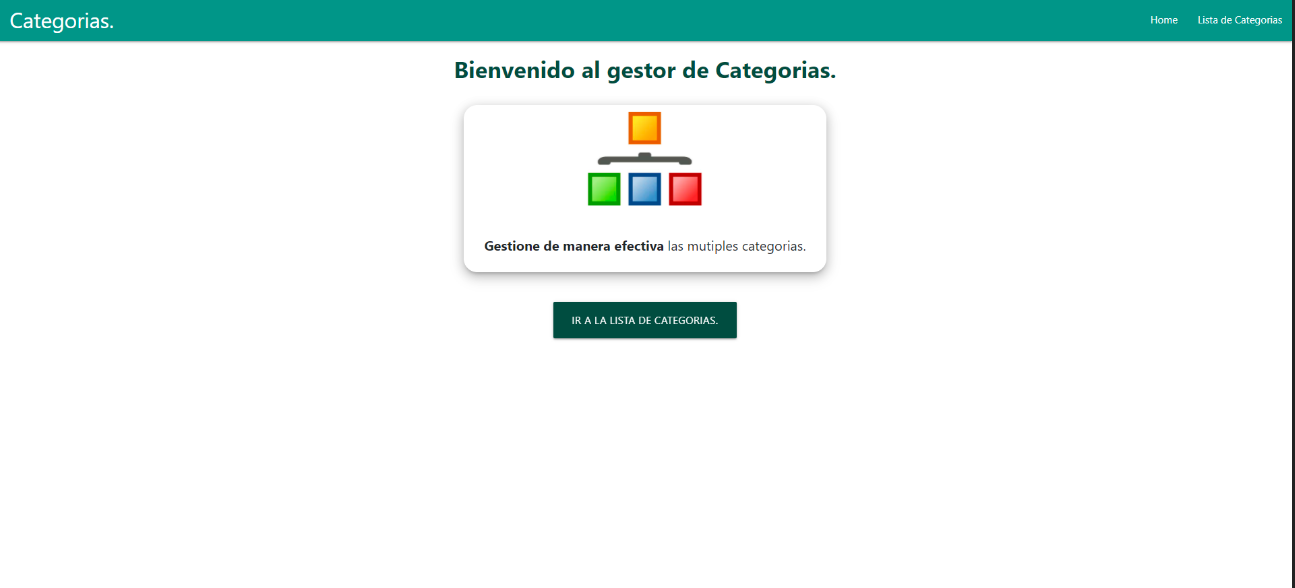
\includegraphics[width=12cm]{2}
\caption{Imagen 2.}
\label{fig:figure1}
\end{figure}
\vspace{60mm}

A continuación podemos ver la imagen con el listado de nuestras categorías, para lo cual hemos implementado dos de ellas alguna que habían sido editadas o modificadas de manera previa para poder probarlo y también otras muchas habían sido eliminadas para poder verificar el funcionamiento del programa, pero en términos generales este es el diseño y también es la manera en que se presenta la lista de categorías a nuestros usuarios por lo cual en mi opinión resulta una interfaz bastante intuitiva y ademas de ello cómoda la vista ya que no es necesario forzar demasiado la vista para poder apreciar los detalles que tiene la práctica y que tiene la interfaz misma además de que los botones representan ya sea un color para ingresar y otro color para borrar el cual esta de color rojo para alertar al usuario de que se trata de una función permanente la cual probablemente no será revertida en esta versión ya que nos echó la implementación para revertir el borrado, pero que sí tendrá cierto impacto o en los datos que se almacenan en nuestra base de datos que previamente hemos diseñado.

\begin{figure}[h]
\centering
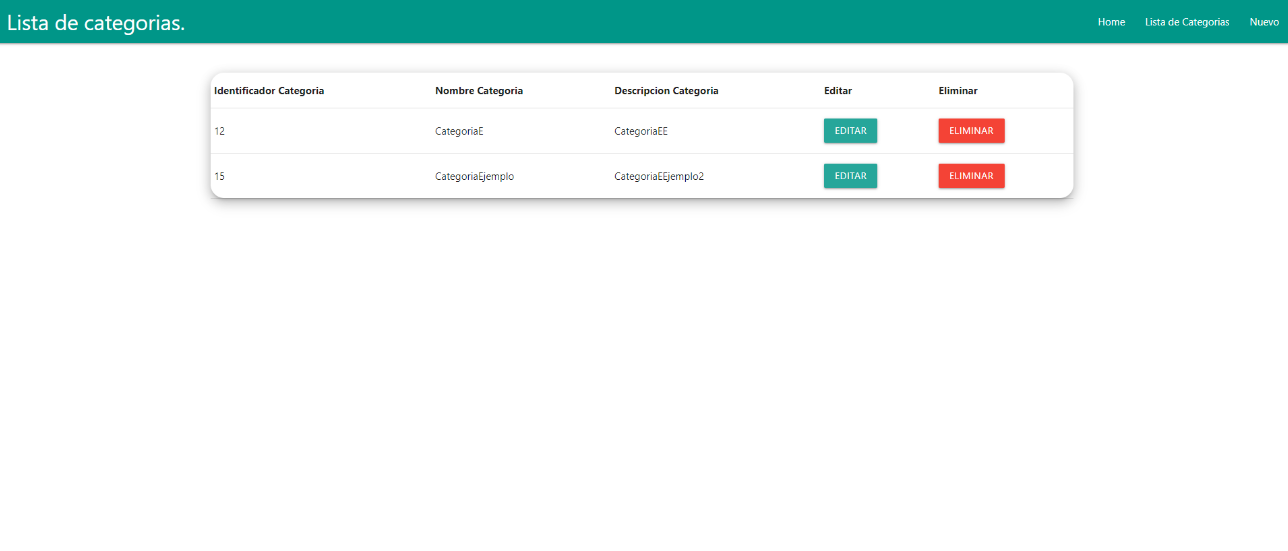
\includegraphics[width=13cm]{3}
\caption{Imagen 3.}
\label{fig:figure1}
\end{figure}

En la siguiente imagen podemos apreciar, el formulario que sea utilizado para poder implementar las actualizaciones de las categorías, como se mencionó el grado de validación dependerá precisamente de las necesidades del cliente o sobre todo en las consideraciones que el desarrollador tenga como para lo cual hemos implementado algunos cuantos validaciones bastante simples, pero efectivas, por lo cual podemos apreciar también el paradigma de diseño de Google implementado nuestro formulario para mantener la estética constante además de que tiene un color verde asimilando el botón que previamente se había presionado con la intención de poder ingresar alguna nueva categoría o poder en este caso editarla.

\begin{figure}[h]
\centering
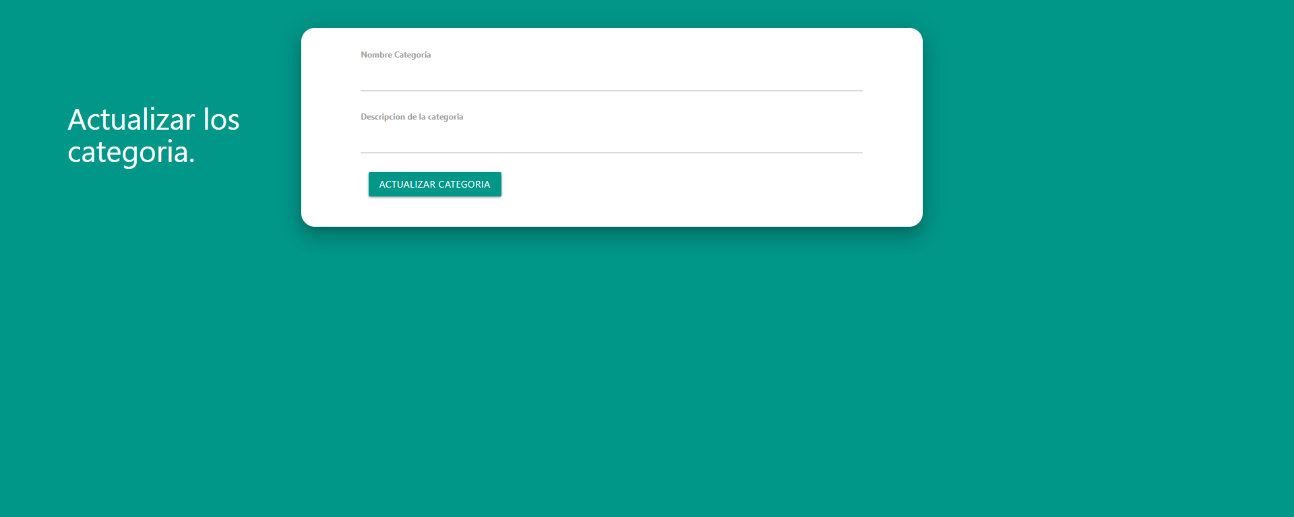
\includegraphics[width=13cm]{4}
\caption{Imagen 4.}
\label{fig:figure1}
\end{figure}

\vspace{60mm}


Posteriormente podremos apreciar que también tenemos el formulario para poder insertar todo lo referente a nuestras nuevas entradas y poder con ello mostrar en pantalla posteriormente en la lista de categorías toda nuestra categoría resultante, por lo cual este sencillo pero bastante efectivo diseño resulta muy concordante con lo que ya hemos presentado anteriormente por el usuario no se siente despistado al tener o formular evitar mucho por lo cual ahora es bastante sencillo simplemente tener los datos y poder ingresar los para tener la categoría que se desea.

\begin{figure}[h]
\centering
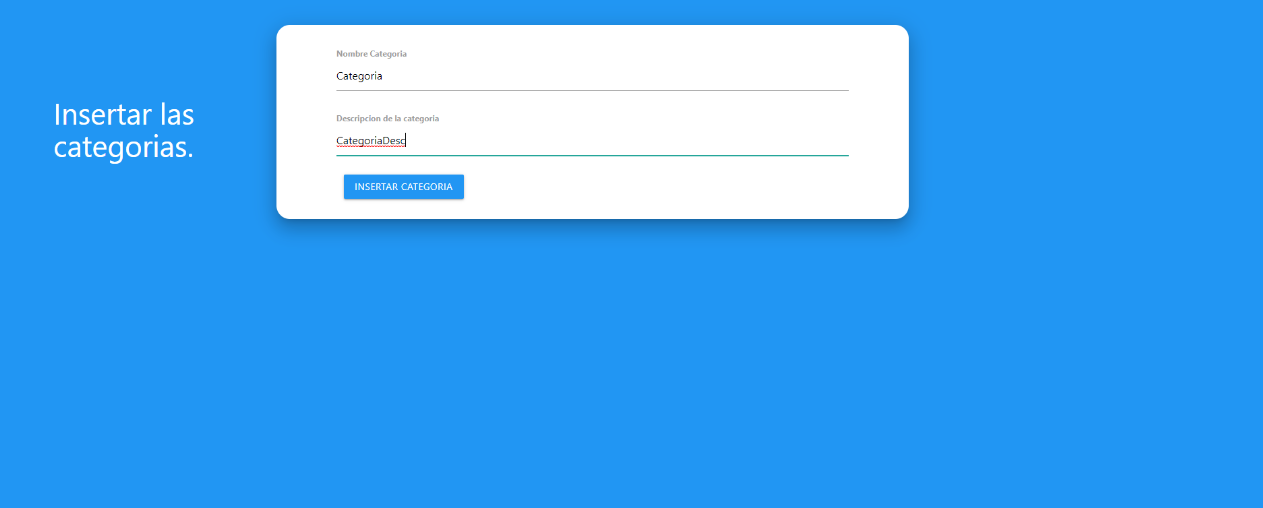
\includegraphics[width=13cm]{5}
\caption{Imagen 5.}
\label{fig:figure1}
\end{figure}

Una vez que ya hemos presentado esta parte cabe mencionar que también cuando nosotros damos click sobre las categorías creadas, podemos desplegar los datos a través de simples tarjetas gráficas las cuales facilitan bastante poder apreciar la información de manera muy sencilla en una tarjeta gráfica Padre lo cual hace que el usuario no se sienta despistado al ver los datos y ademas de ello tienen información organizada en la Palma de su mano ya que es mucho más sencillo poder apreciar todo de forma mucho más dinámica además de que en mi opinión el modelo de tarjetas gráficas ayuda bastante a poder adaptar la información a dispositivos móviles sin importar el tamaño de pantalla con lo cual esto podría ser una tremenda ventaja en términos de responsividad en el diseño.
\begin{figure}[h]
\centering
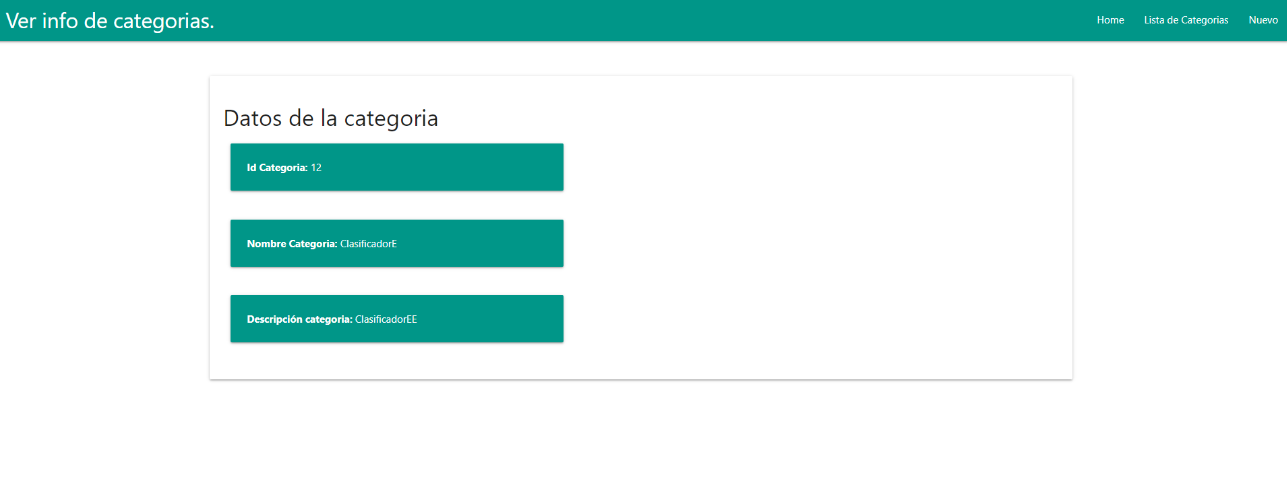
\includegraphics[width=13cm]{6}
\caption{Imagen 6.}
\label{fig:figure1}
\end{figure}

\vspace{60mm}

Ahora posteriormente hemos de mostrar la página con el código de error, la cual simplemente muestra que hay algún tipo de error el cual impide hacer alguna acción, este tipo de ventanas es bastante útil ya que nos ayudan a poder indicar de manera efectiva que algo no anda bien con lo cual es mucho más sencillo darse cuenta de que es el problema y sobre todo como poder atender dicho problema para poder tener un funcionamiento correcto es satisfactorio del sistema y del mismo modo éste pueda cumplir de forma cabal su propósito principal.

\begin{figure}[h]
\centering

\includegraphics[width=13cm]{7}
\caption{Imagen 7.}
\label{fig:figure1}
\end{figure}

A continuación, como ya hemos presentado la interfaz de manera directa, quiero destacar que el diseño de la base datos cumple de manera exitosa en su propósito inicial todo lo que se ha planteado, por lo que desde la creación de ciertas rutinas que habíamos hecho a través de la consola del gestor de base de datos se pudo implementar todo forma muy muy rápida, lo cual para mí bastante satisfactorio porque ahorro bastante trabajo en la parte diseño de base de datos aunque a decir verdad también en un diseño sumamente sencillo pero como se mencionó en un principio bastante funcional y que cumple trabajo a la perfección.
\begin{figure}[h]
\centering
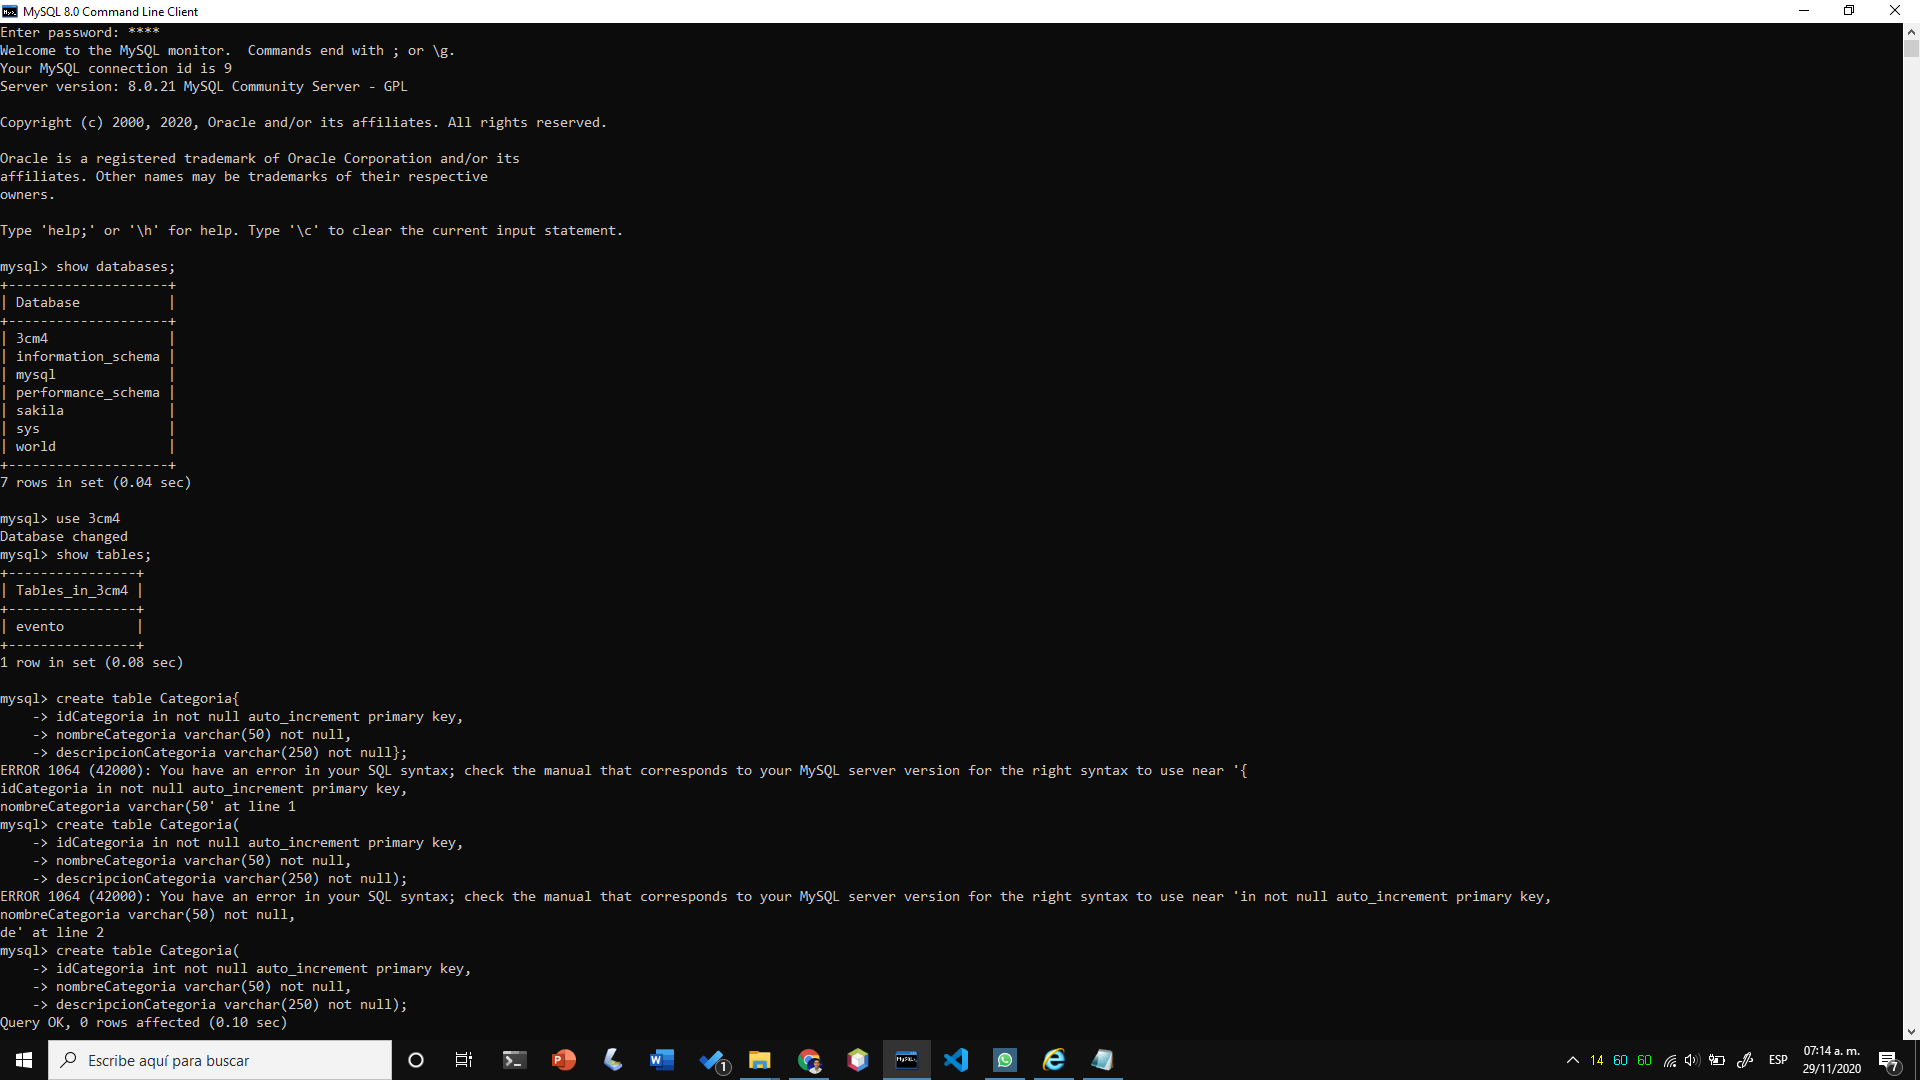
\includegraphics[width=13cm]{8}
\caption{Imagen 8.}
\label{fig:figure1}
\end{figure}

\vspace{60mm}

Ahora vale la pena mencionar que en nuestro proyecto o primero que nada tuvimos que haber sentado las bases para lo cual analizaremos la siguiente serie de archivos con su código para poder mostrar de manera próxima da como es su funcionamiento y poder tener una mejor idea de como éste fue implementado para el trabajo posterior con nuestros jsp, los cuales ya tienen una interacción un poco más directa con lo que del cliente.

\begin{figure}[h]
\centering
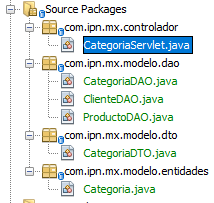
\includegraphics[width=5cm]{9}
\caption{Imagen 9.}
\label{fig:figure1}
\end{figure}

Tenemos el archivo de categoría, que nos ayuda a poder hacer las definiciones de los ya bien conocidos getter y setter que utilizará nuestro programa a lo largo del desarrollo de toda la práctica, por lo cual se considera esto bastante importante, pero debemos tener en consideración que todos los nombres y declaraciones queramos deben tener total coherencia con la parte que ya hemos implementado de forma previa en nuestra base de datos, ademas de ello en el análisis posterior de algunas cuantas imágenes con código se mostrará también la configuración que se hizo directa en el servidor para poder tener una conexión bastante rápida con nuestra base de datos ya generada.
\begin{figure}[h]
\centering
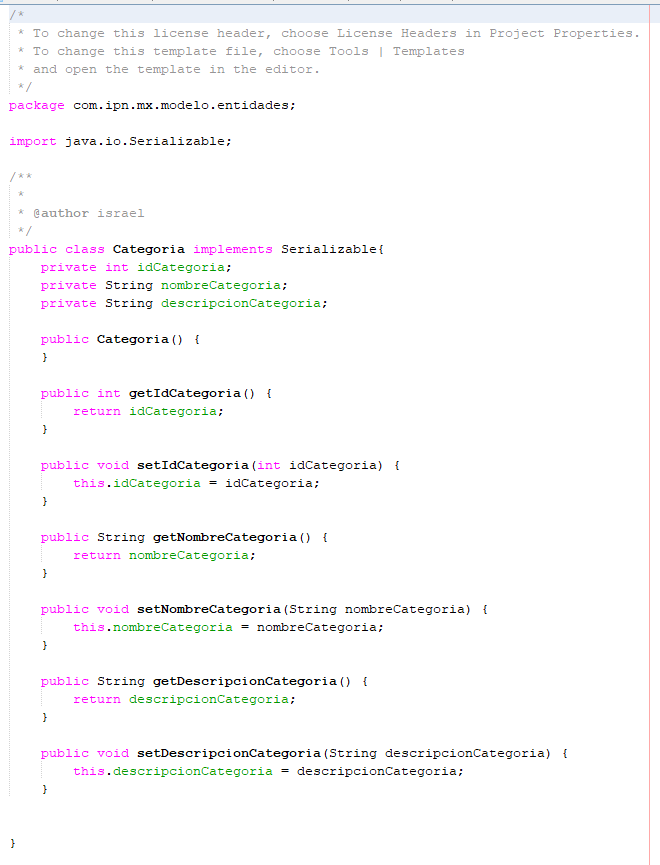
\includegraphics[width=9cm]{Categoria}
\caption{Imagen 10.}
\label{fig:figure1}
\end{figure}

\vspace{60mm}

Ahora en la parte de categoríaDao, del mismo modo tenemos algunas contras definiciones básicas pero también hay que destacar que hemos hecho algunas definiciones para poder generar sentencias en el lenguaje de SQL, con lo cual es mucho más sencillo poder generar un interacción más dinámica con nuestra base de datos lo cual en un futuro nos facilita bastante la tarea de poder hacer que la interfaz interactúe con el backend.

\begin{figure}[h]
\centering
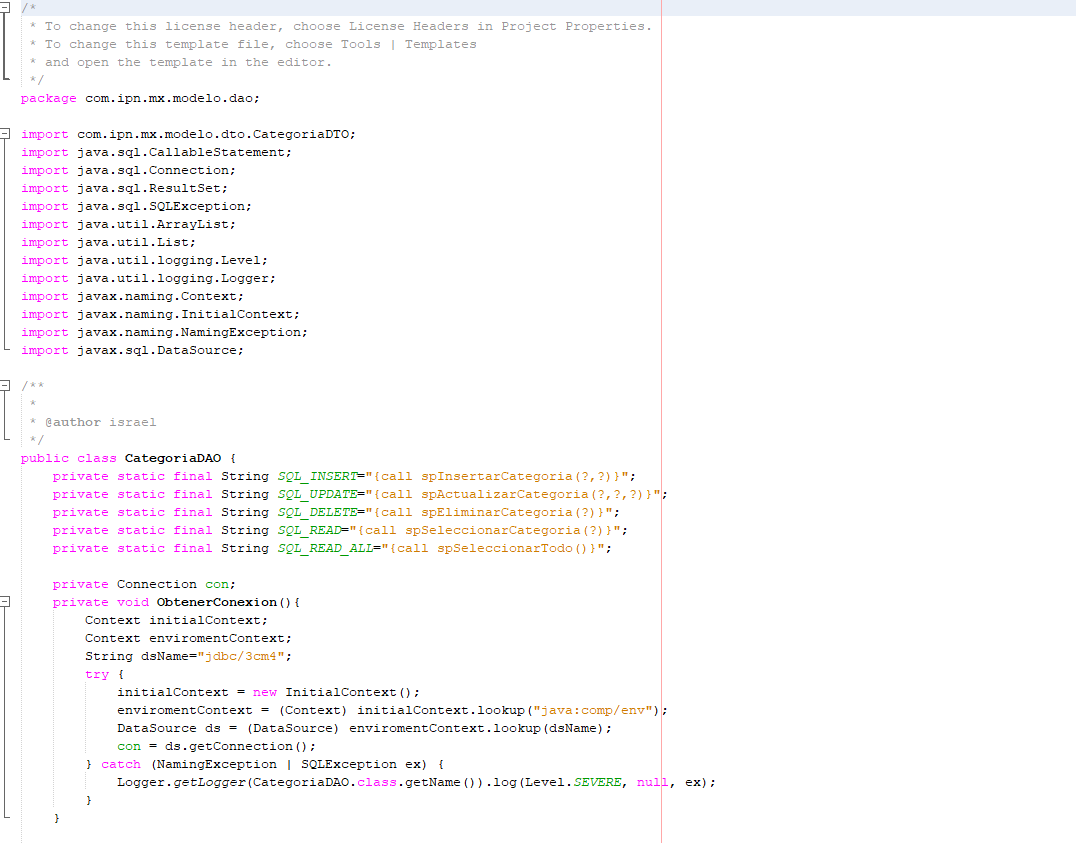
\includegraphics[width=9cm]{CategoriaDao1}
\caption{Imagen 11.}
\label{fig:figure1}
\end{figure}

Seguido de ello se puede ver cómo queríamos algunas de las validaciones que necesitamos para poder disparar algunas excepciones que se generen durante cierta parte de la conexión o de la llamada de cierta sentencias para el manejo de nuestra base de datos, lo cual es bastante importante porque nos ayuda a garantizar la calidad de la conexión además de que también podemos garantizar la calidad de las operaciones que se realicen y sobre todo tener ciertas certeza de que la funcionalidad se llevará a cabo de forma totalmente satisfactoria y con mucha facilidad sobre todo.
\begin{figure}[h]
\centering
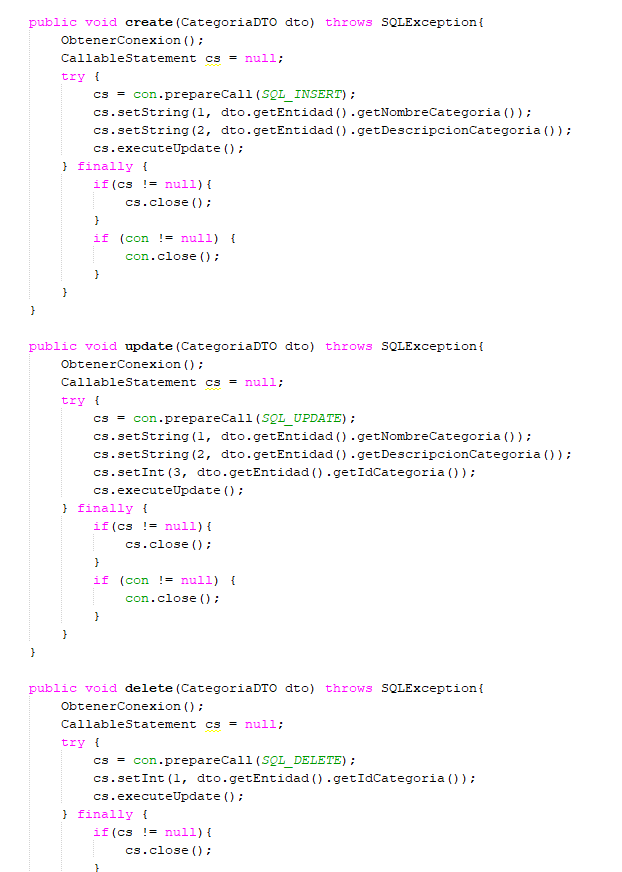
\includegraphics[width=6cm]{CategoriaDao2}
\caption{Imagen 12.}
\label{fig:figure1}
\end{figure}

\vspace{60mm}

En esta siguiente parte como se mencionó también se seguirán haciendo algunos cuantos validaciones para poder mantener la calidad y sobre todo garantizar que la conexión se va llevar a cabo de la manera en que nosotros lo buscamos y que no haya ningún problema al momento de interactuamos de manera concreta con nuestra base de datos.

\begin{figure}[h]
\centering
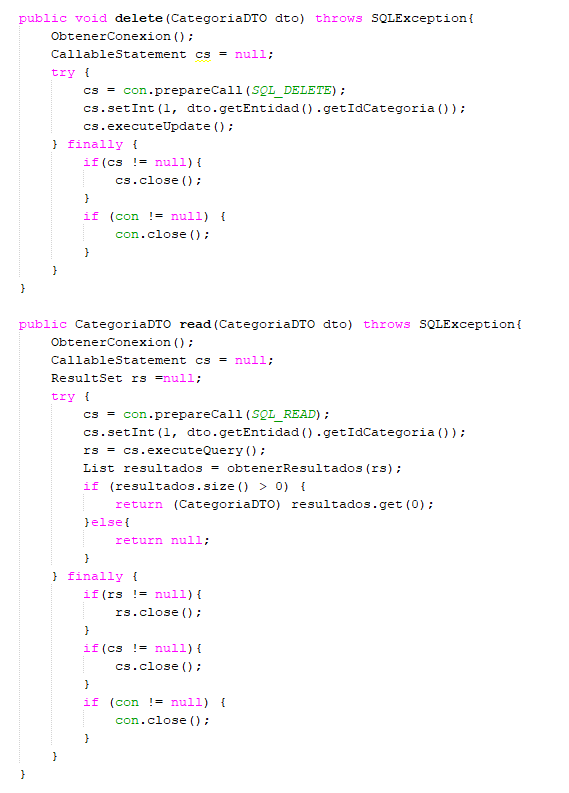
\includegraphics[width=7cm]{CategoriaDao3}
\caption{Imagen 13.}
\label{fig:figure1}
\end{figure}

Ahora bien, podemos ver también como tenemos la lectura de toda la lista y de manera posterior también como hacemos la obtención de los resultados precisamente de nuestra base de datos haciendo referencia precisamente a los campos que ya habíamos definido de forma previa durante la parte del explicación teórica entre los cuales se pueden ver el identificador, el nombre de la categoría y ademas de ello la descripción de la categoría, lo cual como ya lo mencione de forma previa nos ayudara a facilitar muchísimo la conexión entre lo que el cliente de y la base de datos.
\begin{figure}[h]
\centering
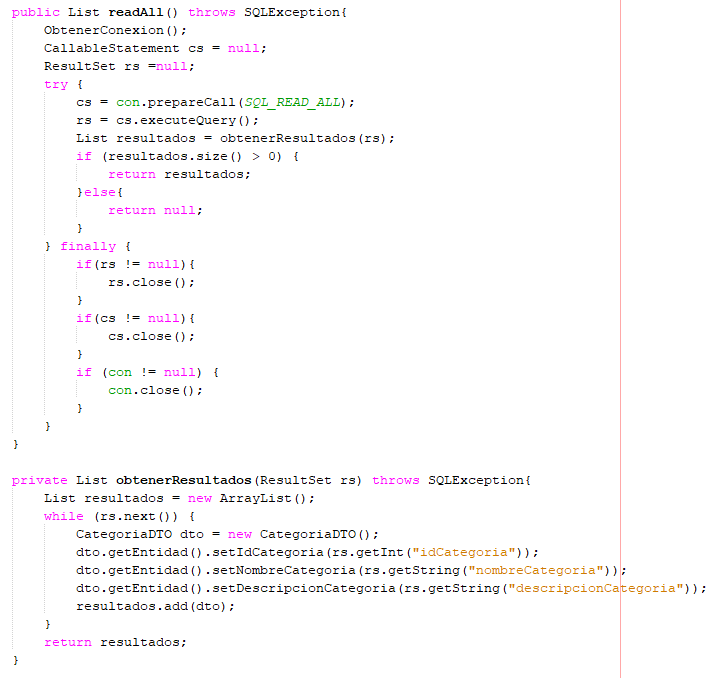
\includegraphics[width=7cm]{CategoriaDao4}
\caption{Imagen 14.}
\label{fig:figure1}
\end{figure}

\vspace{60mm}

Posteriormente hay que destacar, que se ha trabajado también con esta parte van a poder como se mencionó agilizar muchísimo más el trabajo con la base de datos, aunque a decir verdad este es un código mucho más corto pero que en parte llave sido implementado la practica uno pero que ahora ha sido adaptado para poder lidiar con el trabajo de la gestión de las categorías.

\begin{figure}[h]
\centering
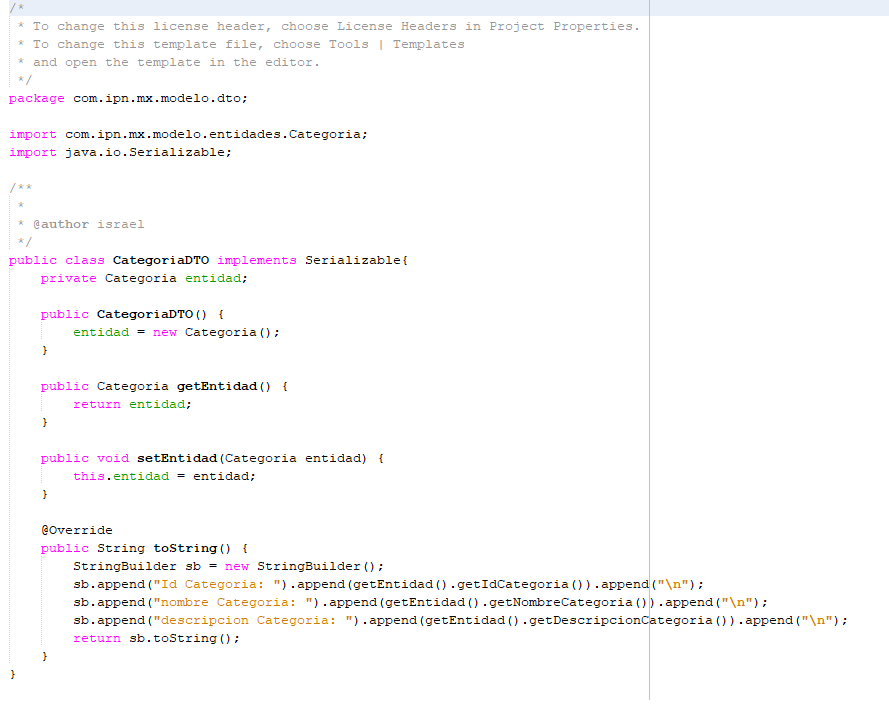
\includegraphics[width=12cm]{categoriaDTO}
\caption{Imagen 15.}
\label{fig:figure1}
\end{figure}

Ahora también tenemos la parte del servlet que en un principio de la práctica habíamos creado con otro nombre pero que fue evitado con fines prácticos para poder identificar mucho mejor la interacción que este tiene directamente con las categorías, para lo cual de inicios hacen algunas importaciones básicas y esenciales para el correcto funcionamiento, las cuales son gestionadas precisamente por nuestro entorno de desarrollo y que deben estar presentes para que pueda funcionar a plenitud el software que estamos diseñando.
\begin{figure}[h]
\centering
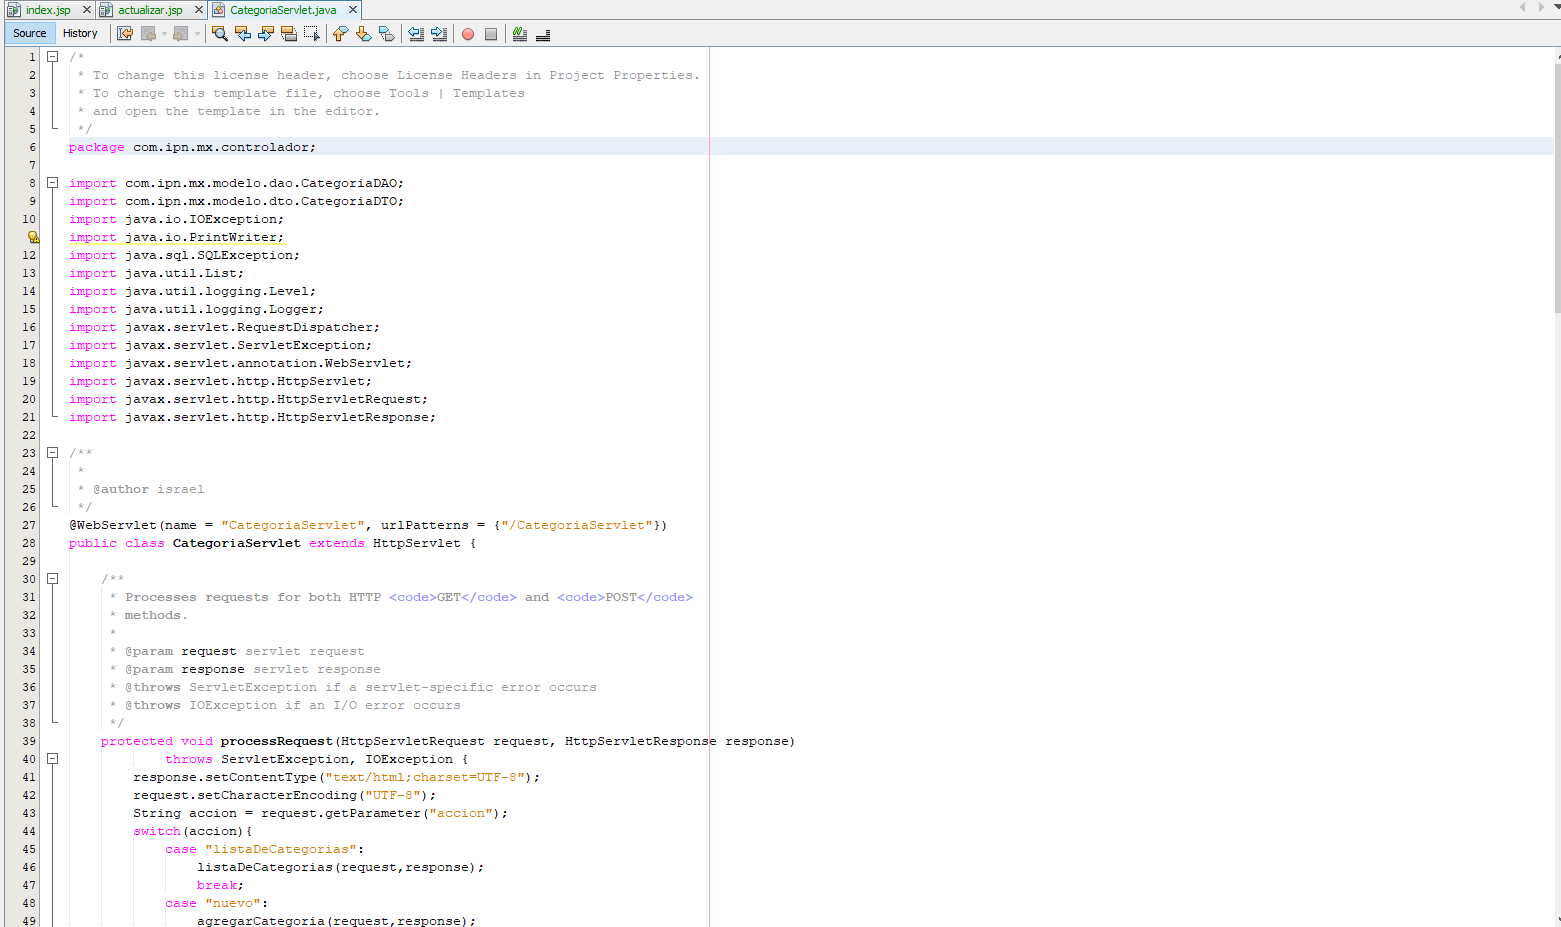
\includegraphics[width=10cm]{categoriaServlet1}
\caption{Imagen 16.}
\label{fig:figure1}
\end{figure}

\vspace{60mm}

Si bien en la siguiente parte mostramos la implementación de múltiples casos en los cuales podemos apreciar de forma directa como se han definido algunas de las funciones principales con las que contará nuestro sistema en un futuro y con el que precisamente el usuario interactúa la directamente en la interfaz, y también tenemos la parte de la lista de gato y varias la cual no ser bastante útil para poder tener en concreto todo el despliegue de las mismas.

\begin{figure}[h]
\centering
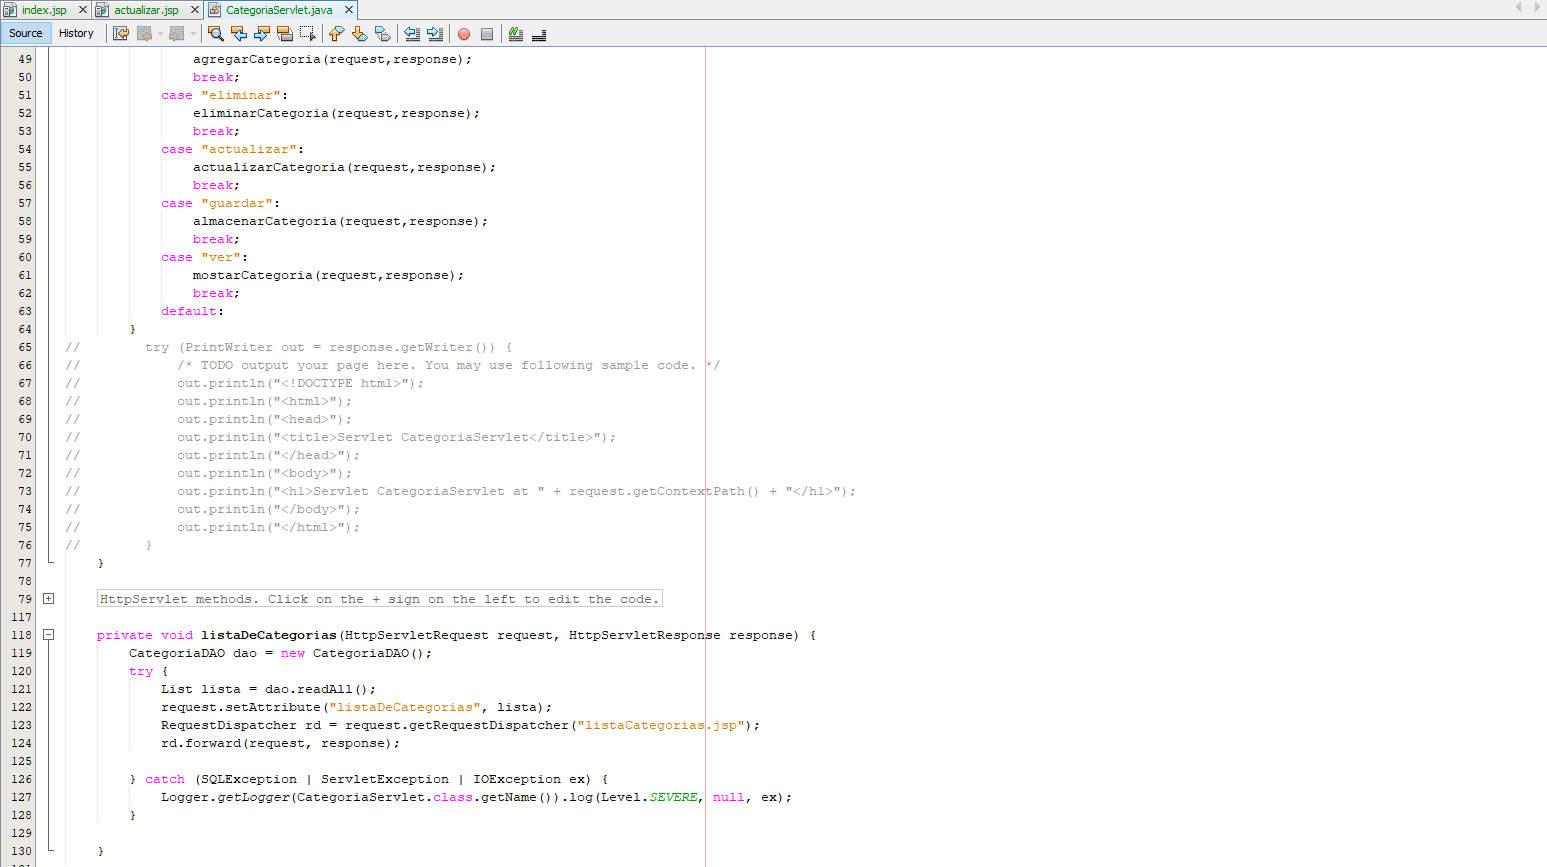
\includegraphics[width=12cm]{categoriaServlet2}
\caption{Imagen 17.}
\label{fig:figure1}
\end{figure}

Ahora en la tercera parte lo que podemos ver es que también se hace mención de la función de agregar categorías, eliminar categorías, actualizar las categorías, almacenar las categorías y finalmente poder a mostrar o ver las categorías directamente en nuestras tarjetas gráficas como lo mencione en un principio, con el fin de que el usuario se sienta bastante cómodo al poder apreciar a toda la información recolectada de las categorías que la creado, pero en este caso en este código estamos prácticamente sentando las bases para que podamos interactuar de forma directa con la base datos y todo el código o de una manera modular de forma que si en un futuro lo deseamos podamos escalar nuestro proyecto o a niveles que probablemente en un principio no saben considerado pero que ahora gracias y debido a la capacidad instalada aumentada podría ser de bastante utilidad para poder cubrir necesidades a una escala superior o inclusive por qué no decirlo también en ciertas circunstancias poder cubrir necesidades a una escala inferior pero que todo el software se mantenga siempre de forma modular para poder trabajar y desde luego siendo esto o parte de la calidad del software también se debe considerar que debe ser flexible y sobre todo tener ese grado de escalabilidad.
\begin{figure}[h]
\centering
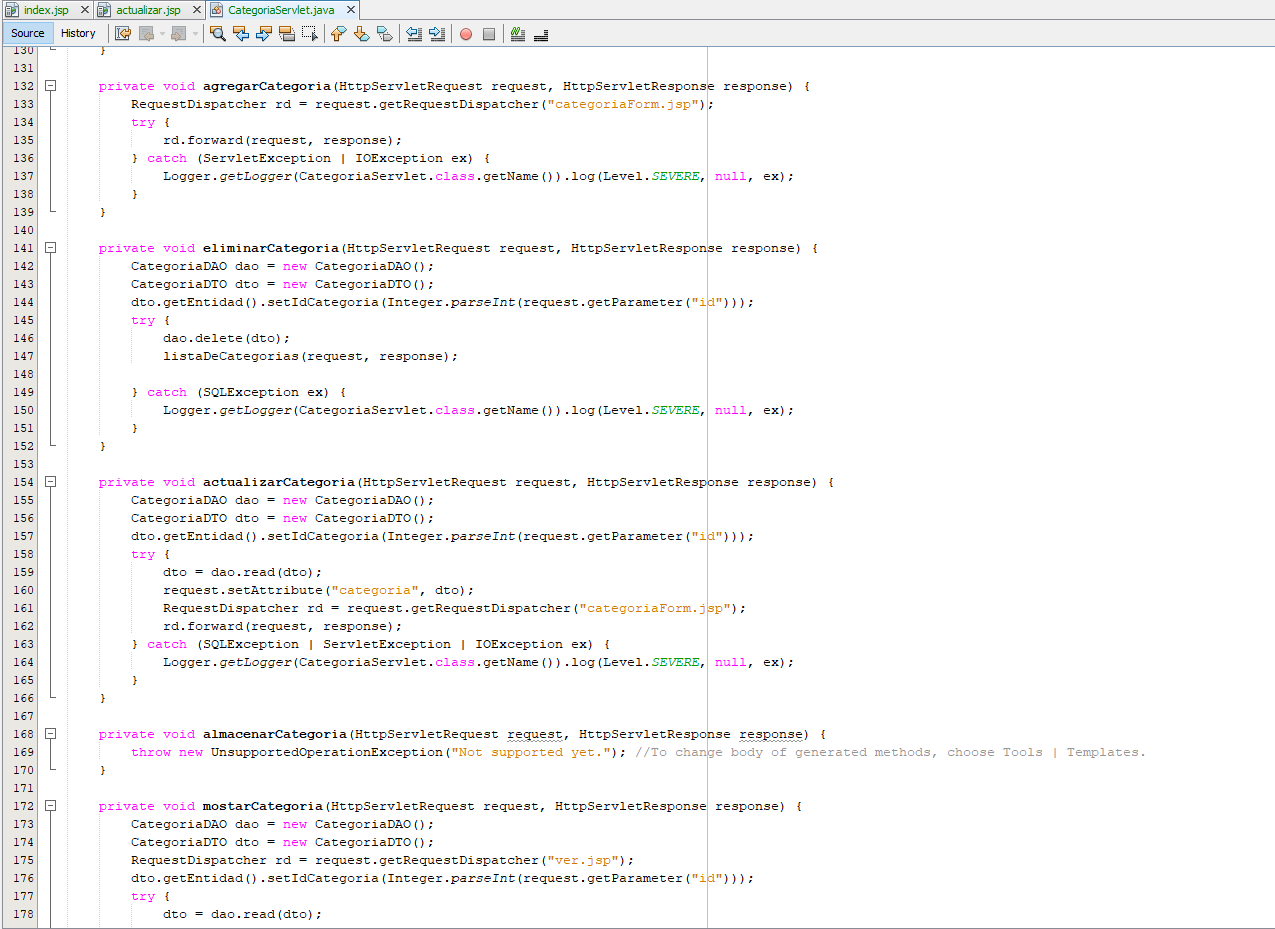
\includegraphics[width=10cm]{categoriaServlet3}
\caption{Imagen 18.}
\label{fig:figure1}
\end{figure}

\vspace{60mm}

Ahora pasando la parte del cliente podemos ver que también hemos hecho parte de la conexión que nos correspondía con la base de datos que ya previamente es generamos, la cual en el nombre de nuestro grupo pero también tiene como definiciones principales algunas de las consultas básicas que se pueden hacer para nuestra base de datos, cabe destacar que hemos utilizado el signo de interrogación con la finalidad de poder recibir cualquier tipo parámetro que evidentemente está asociado a es identificador específico de la base datos que ya hemos definido en nuestro gestor de base de datos.

\begin{figure}[h]
\centering
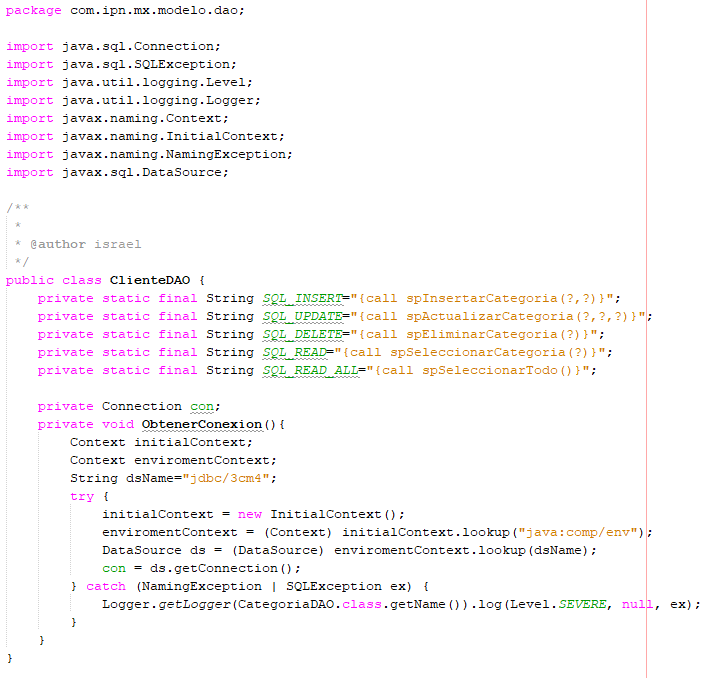
\includegraphics[width=8cm]{clienteDao}
\caption{Imagen 19.}
\label{fig:figure1}
\end{figure}

Y en la parte del producto dao ocurre algo muy similar, en realidad como se mencionó este código ya estaba basado en lo de la practica uno, pero aquí la diferencia que hemos hecho es la implementación precisamente de la interfaz y de las funciones además también de la variante en la conexión directa con nuestra base datos como por lo cual se aprecia una evolución en este aspecto.
\begin{figure}[h]
\centering
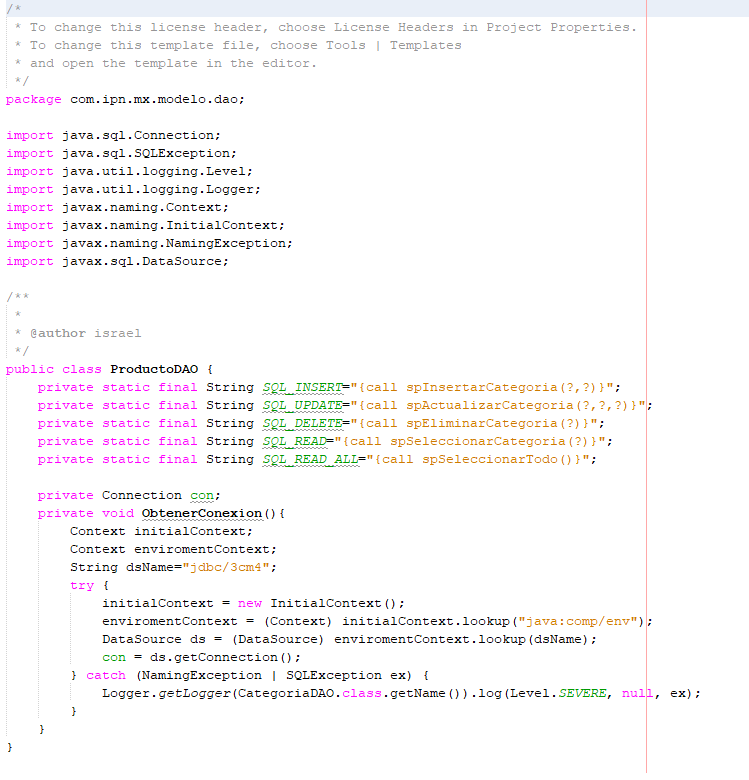
\includegraphics[width=8cm]{productoDao}
\caption{Imagen 20.}
\label{fig:figure1}
\end{figure}

\vspace{60mm}

En esta siguiente imagen podemos apreciar la sección de archivos remotos, no hay que menospreciar esta parte ya que muchas de las cdn nos ayudan a tener lo mejor de código de terceros implementado nuestra idea de software, sin tener que precisamente trabajar en lo mismo o tener que inclusive reinventar la rueda, como se aprecia ahí tenemos dos frameworks, pero en realidad el que estamos utilizando más por convención y la verdad por elección propia es materialize ya que como lo mencione es actualmente el paradigma de diseño frontend más popular ya que está impulsado por la mismísima Google.

\begin{figure}[h]
\centering
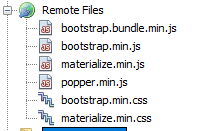
\includegraphics[width=8cm]{10_descripciondirectorio}
\caption{Imagen 21.}
\label{fig:figure1}
\end{figure}

Ya por ultimo lo que vale la pena destacar la implementación que hemos hecho para poder hacer la conexión con la base datos de forma anticipada durante el desarrollo de las clases ya que como se mencionó de manera previa es uno o enfoque y una nueva manera de poder realizar esta conexión, con lo cual se puede apreciar que existen distintas maneras y la variedad no puede escasear en este tipo proyectos por lo que sí lo pensamos de forma cautelosa esto puede ser de mucha ayuda ya que es incierto proyectos está trabajando de esta manera nosotros podamos entender de forma concreta que hacer y a donde acceder para poder consultar que tipo de conexión sexta siendo y desde luego en caso de que existe algún error o se deban hacer cambios de manera inminente gracias a las necesidades del cliente nosotros podamos actuar de la manera en que corresponde ante estos cambios y ante estas necesidades por cubrir.
\begin{figure}[h]
\centering
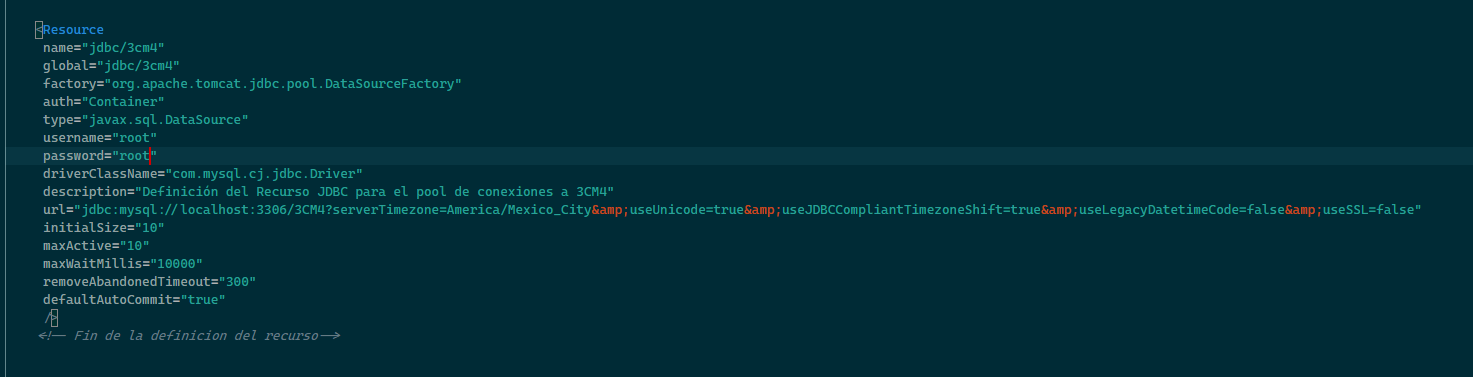
\includegraphics[width=17cm]{10_descripciondirectorio1}
\caption{Imagen 22.}
\label{fig:figure1}
\end{figure}

\vspace{300mm}

Ya para terminar con la descripción, es destacable que también hemos modificado nuestra chupó de contexto para poder establecer una conexión exitosa con la referencia que hemos generado con el JDBC para la conexión de nuestra base de datos como para lo cual deberemos describir de forma exacta el nombre de nuestra base de datos como le hemos definido de manera previa en nuestro gestor, lo cual a decir verdad no es gran ciencia si ya conocemos como es que funciona la sintaxis y ademas de ello ya hemos configurado de manera previa nuestro servidor o en este caso las configuraciones del servidor que estamos se plantó, las cuales variarán de cuando en cuando dependiendo del fabricante o en este caso de la empresa que lo distribuya o del tipo de servidor que se trate.
\begin{figure}[h]
\centering
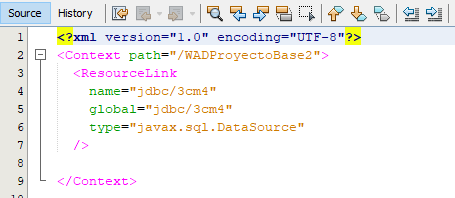
\includegraphics[width=13cm]{10_descripciondirectorio2}
\caption{Imagen  23.}
\label{fig:figure1}
\end{figure}

\pagebreak

%################################################
\section{\color{colorIPN}{Resultados}}

Como resultado de esta práctica, se ha logrado tener un sistema que cumpla con los requerimientos mínimos para poder hacer implementaciones y gestión sencilla de categorías, las cuales pueden ser creadas por el usuario y almacenadas en nuestra base datos para su posterior manejo inicialización, por lo como ya ha lanzado un panel prevé quedó bastante satisfecho con los resultados de esta práctica por las posibilidades que ofrece en futuros desarrollos y además muestra de forma muy certera como es que se pueden hacer este tipo de implementaciones de forma bastante sencilla, modular, práctica y sobre todo muy eficiente ya que en unas cuantas líneas de código se puede hacer una interacción muy robusta para que el usuario puedan realizar múltiples tareas a través del sistema.
\vspace{5mm}
Uno de los aspectos en los que me enfoque también en esta práctica es en el desarrollo un interfaz que fuera cómoda y legible para el usuario, en la cual él no se sintiera perdido entre la variedad de opciones que la ofrecemos y puede intuir de manera muy simple como es que el sistema funciona y todas las posibilidades que estén ofrece en el camino.
\vspace{5mm}
Para lo cual yo considero que esta parte es fundamental porque no solamente es la carta de presentación del sistema, sino que también da la sensación de que es un software que no solamente en la parte del backend está programado con calidad sino que también ofrecen funcionalidad es un tanto más avanzadas, aunque en realidad las funcionalidades cofre se son bastante estándar pero no por ello son peores sino que ayudan a realizar actividades básicas de una forma en la que ha sido implementado con una estructura que permite en un futuro poder hacer más escalable este proyecto, y que ademas como lo mencione de forma previa también nos da la pauta para poder escribir nuestro código de la manera en que nosotros queramos, realizar las conexiones a bases de datos de la forma en que nuestros lo deseamos, y también poder implementar distintos códigos de terceros que nos ayuden a realizar nuestra labor de forma mucho más eficiente y sobre todo ofrecer soluciones en velocidades record.

\begin{figure}[h]
\centering
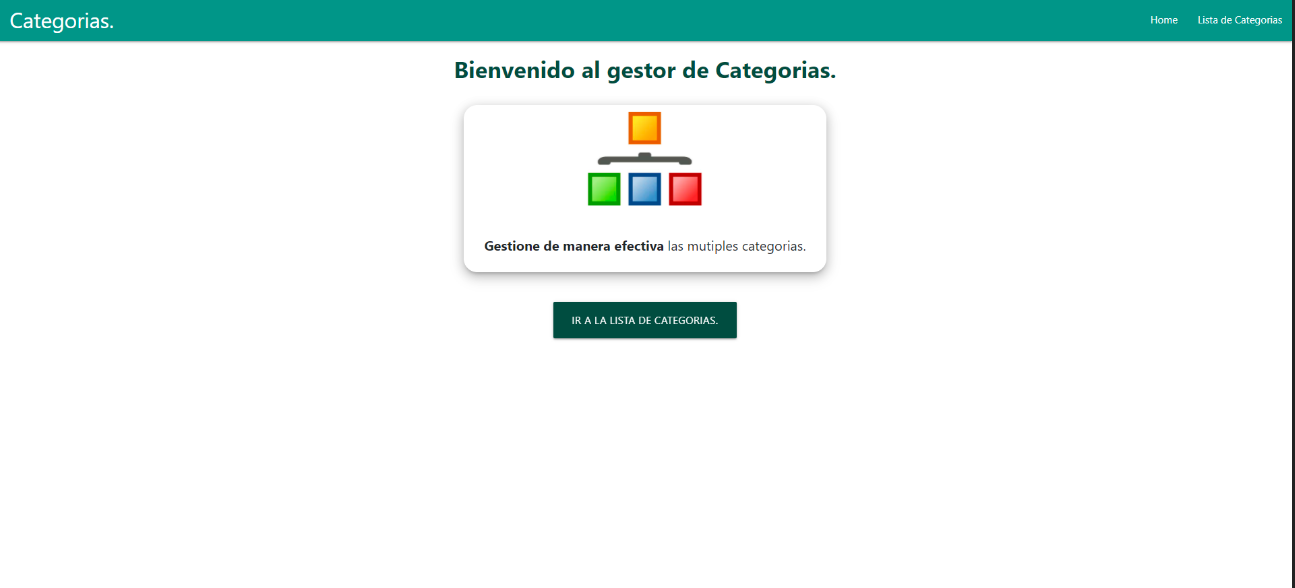
\includegraphics[width=13cm]{2}
\caption{Vista del resultado.}
\label{fig:figure1}
\end{figure}



\pagebreak


%################################################
\section{\color{colorIPN}{Conclusión}}

Puedo concluir, que en esta practica he aprendido muchísimas cosas sobre como implementar funcionalidades básicas que a pesar de que son básicas, se presentan de manera contundente una manera simple de poder hacer implementaciones de forma bastante rápida en sistemas que funcionan a un nivel bastante realista y que pueden ofrecer soluciones muy buenas a ciertos usuarios con necesidades específicas, en este caso al nosotros estar enfocados en prácticas que tienen que ver con la gestión de datos y en este caso funcionalidades bastante simples pero muy necesarias, podemos darnos una idea de como es que se debe trabajar en términos de las aplicaciones web y también como es que esta nos permiten ofrecer una facilidad enorme para el diseño de interfaces que son mucho más intuitivas y que se adaptan a lo que el cliente nos pida o inclusive a el desarrollo o solución que queramos implementar.

\vspace{5mm}

La verdad es que he de decir que estoy bastante emocionado por las posibilidades que esto ofrece, pero también me quedo hasta cierto punto sorprendido por la gran variedad de formas que hay para desarrollar un mismo proyecto o o desarrollar un idea similar, ya que usualmente en el desarrollo tradicional suele ser bastante estándar la manera en que se hacen ciertas cosas, a menos de quiera se utilizan otras herramientas que el mercado te permiten hacer trabajo asíncrono o inclusive evitar tiempos de carga, pero en General el desarrollo web tradicional siempre se visten pensado por las venas corrientes y del mismo modo también se siguen patronal muy específicos; pero en el caso del trabajo con el lenguaje de programación JAVA se tienen buenos resultados además de que también se puede conseguir una flexibilidad bastante amplia respecto a la manera en que se pueden solucionar los problemas o inclusive los paradigmas que pueden ser implementados para llegar a ciertas soluciones.

\vspace{5mm}

Algo que pudo decir que disfrute bastante de la práctica, es trabajar desde luego con la parte de la interfaz de usuario, porque yo considero que es una de las secciones más importantes pero además también pienso que debe haber una buena implementación del backend para poder entonces tener una interfaz que realmente esa dinámica y que realmente a la sentido para el usuario y que le permita trabajar de una manera mucho más cómoda y por qué no decirlo inclusive mucho más intuitiva que haga la experiencia de uso entrañable.
\vspace{5mm}

Me quedo con un muy buen sabor de boca por esta práctica, y del mismo modo bastante ansioso por saber qué es lo que deben de la para el desarrollo de nuestro proyecto o y de futuras prácticas para las siguientes unidades, algo que también me gustaría conocer es hasta qué punto que podemos inclusive hacer implementaciones de esta manera y también entender un poco más sobre las limitantes inclusive las ventajas que alguna de ellas nos ofrecen respecto a otras maneras de trabajar, pero supongo que esos un aspecto que se irá viendo a lo largo del tiempo conforme con la experiencia serán ciertas implementaciones que me permitan poder apreciar esto con mucho mayor claridad y sobre todo por ver en tiempo real como es el funcionamiento del software o de la solución que se está ofreciendo a el cliente o a la necesidad en concreto.

\pagebreak

%################################################

\section{\color{colorIPN}{Referencias Bibliográficas}}
\color{colorESCOM}{
	\begin{thebibliography}{10}
	
		\bibitem[GeeksforGeeks, 2020]{GeeksforGeeks}
		Introduction to JSP
		\newblock {\em https://www.geeksforgeeks.org/introduction-to-jsp/}
		\newblock GeeksforGeeks, 2020.

\bibitem[jtech, 2020]{jtech}
		jtech
		\newblock {\em http://www.jtech.ua.es/j2ee/2006-2007/doc/sesion08-apuntes.pdf}
		\newblock jtech, 2020.

	\end{thebibliography}
}

\end{document}
